%%%%%%%%%%%%%%%%%%%%%%%
%%% Document Set up %%%
%%%%%%%%%%%%%%%%%%%%%%%

\documentclass[11pt]{amsart}


% you can add extra packages if you need them
\usepackage{amsfonts, amssymb, amscd, amsmath, amsthm, enumerate, verbatim, calc, 
thumbpdf, mathrsfs, graphicx, multicol, tabu, tikz}

\setlength{\oddsidemargin}{0.25in}  % please do not change
\setlength{\evensidemargin}{0.25in}  % please do not change
\setlength{\marginparwidth}{0in}  % please do not change
\setlength{\marginparsep}{0in}  % please do not change
\setlength{\marginparpush}{0in}  % please do not change
\setlength{\topmargin}{0in}  % please do not change
\setlength{\footskip}{.3in}  % please do not change
\setlength{\textheight}{8.75in}  % please do not change
\setlength{\textwidth}{6in}  % please do not change
\setlength{\parskip}{4pt}  % please do not change


\theoremstyle{plain}  % default
\newtheorem{thm}{Theorem}[section]
\newtheorem{lem}[thm]{Lemma}
\newtheorem{cor}[thm]{Corollary}
\newtheorem{prop}[thm]{Proposition}
\newtheorem{mythm}[thm]{My Great Result}

\theoremstyle{definition}
\newtheorem{defin}[thm]{{Definition}}
\newtheorem{ex}[thm]{Example}

\theoremstyle{remark}
\newtheorem{rem}[thm]{Remark}
\newtheorem*{note}{Note}
\newtheorem{case}{Case}

\numberwithin{equation}{thm}

\newcommand{\dims}{\operatorname{dims}}
\newcommand{\rank}{\operatorname{rank}}

\DeclareMathOperator{\lcm}{lcm}

\usetikzlibrary{arrows}



%%%%%%%%%%%%%%%%%%%%%%%%%%%%%%%%%
%%% Document Meta Information %%%
%%%%%%%%%%%%%%%%%%%%%%%%%%%%%%%%%


\begin{document}


\title[Abstract Algebra Project]{Investigation of resolving sets and metric dimension}
\thanks{Dogan Comez}
\author[K.~ R. Ryan]{Kyle Ryan\\{Advisors: Trevor McGuire, Warren Shreve}}


\address{Department of Mathematics 2750\\ North Dakota State University\\PO BOX 6050\\ Fargo, ND 58108-6050\\ USA}

\email{kyleryanmn@gmail.com, trevor.mcguire@ndsu.edu, warren.shreve@ndsu.edu}





\maketitle
% \setcounter{page}{***} % Please do not change this line


\begin{abstract}
        For any graph G it is possible to describe each of its vertices uniquely with respect to an ordered subset of vertices of G called a resolving set.
    In this project, we investigate properties of associated with minimal resolving sets, known as bases and conditions under which changing G affects its bases. 
\end{abstract}

%%%%%%%%%%%%%%%%%%%%
%%% Introduction %%%
%%%%%%%%%%%%%%%%%%%%

\section{introduction}

    %The basics of what you're doing: relevant tools, defs techniques etc%
    For this investigation we will begin with several basic defintions that might not be part of a typical introduction to graph theory.

 \begin{defin}[Representation of vertex(with respect to W)]:\\
    For an ordered subset $W=(w_1, w_2, ..., w_i, w_{i+1}, ...)$ of vertices in $G$, the representation of a vertex $v \in G$ with respect to $W$ denoted $rep(v/W)$ is: \\
  $rep(v/W)=(d(v,w_1), d(v,w_2), ..., d(v,w_i), d(v,w_{i+1}), ... )$
 \end{defin}
    
 \begin{defin}[Resolving Set]:\\
  An ordered subset $W \subset V(G)$ is called a resolving set of G if\\ $\forall v_1, v_2 \in V(G)$  , $rep(v_1/W) \neq  rep(v_2/W)$.
 \end{defin}
 
 \begin{defin}[Basis of a graph]:\\
  A resolving set $W$ of $G$ is called a $basis\ of\ G$ if for any other resolving set $H$ of $G$, $\mid H\mid \geq \mid W\mid$
 \end{defin}
 
 \begin{defin}[Metric Dimension]:\\
  The metric dimension of a graph $G$ denoted $MD(G)$ is the order of any basis for $G$.
 \end{defin}


Finding the metric dimension or any basis for a graph is currently considered to be an NP-Hard problem. 
Metric dimension is known for some subsets of graphs which will be discussed later, but in general it is very difficult or simply time consuming to determine.
The intent of this paper is to investigate whether there is a set of graphs for which having a known metric dimension allows us to determine metric dimension after adding or removing an edge.
Furthermore we will attempt to investigate what properties of these graphs make it possible to determine metric dimension for them after adding or removing an edge.
\begin{ex}
 The path graph $P_3$ has a metric dimension of 1. Simply calling $W$ the set containing one leaf node of $P_3$ is sufficient to construct a basis for $P_3$.
 By adding any edge to $P_3$, $P_3$ becomes $K_3$ which has a metric dimension of 2.
\end{ex}
 \begin{tikzpicture}[>=stealth',shorten >=1pt,auto,node distance=3cm,
                    thick,main node/.style={circle,draw,font=\sffamily\Large\bfseries}]
  \node[main node] (1) {x};
  \node[main node] (2) [right of=1] {};
  \node[main node] (3) [right of=2] {x};
  \node[main node] (4) [right of=3] {};
  \node[main node] (5) [above of=4] {y};
  \path[thick]
    (1)	edge (2)
    (3) edge (4)
    (4) edge (5)
    (3) edge [-,dashed] (5);
\end{tikzpicture}

%%%%%%%%%%%%%%%%%%%%%%%%%%%%%%%%%%%%%%%%%%%%%%%%%%%%%%%%
%%%%%%%       SECTION 1, B-Encodings          %%%%%%%%%%
%%%%%%%%%%%%%%%%%%%%%%%%%%%%%%%%%%%%%%%%%%%%%%%%%%%%%%%%
\section{encodability of graphs with respect to their bases}


  \begin{defin}[Representation set of a graph]:\\
  The representation set of a graph with respect to a basis $W$ is the set $H=\{r(v/W)\mid v\in G\}$.   
  \end{defin}

  \begin{defin}[Unique Encoding]:\\
   If we can construct a graph $G$ from its representation set $H$ by connecting vertices in $G$ 
   if their representations differ by no more than 1 in each place then we say that $G$ is uniquely encoded by $H$.
   Furthermore we say that $G$ is uniquely encodeable with respect to its basis $W$ or $G$ is enccodable under $W$.
  \end{defin}

\begin{lem}
$G$ is encodable under $W$ if and only if $\ \forall$ nonadjacent $\ v_1,\ v_2\in G$:\\
$\ \exists\ w \in W$ s.t. $\left| d(v_1,w)-d(v_2,w)\right| > 1$ 
\end{lem}
\begin{proof}
Let $G$ be a graph with basis $W$. Let $R$ be the representation set of $G$ with respect to $W$. 
Assume that for some pair of vertices $v_1,\ v_2\ \in G$, $\ \exists\ w \in W$ s.t. $\left| d(v_1,w)-d(v_2,w)\right| > 1$.
If we construct a graph $H$ from $R$ following the encoding scheme descibed above, $v_1,\ v_2$ will be adjacent in $H$. 
Then $H \neq G$ and so $G$ is not encodable under $W$.
\end{proof}

\begin{ex}
Observe the following\\

\begin{tikzpicture}[>=stealth',shorten >=1pt,auto,node distance=3cm,
                    thick,main node/.style={circle,draw,font=\sffamily\Large\bfseries}]
\node[main node] (1) {x};
\node[main node] (2) [above right of=1] {};
\node[main node] (3) [above left of=1] {};
\node[main node] (4) [above of=2] {y};
\node[main node] (5) [above of=3] {};

\path[thick]
  (1) edge (2)
      edge (3)
  (2) edge (3)
      edge (4)
  (3) edge (5);

\node[main node] (8) [right of=2] {x};
\node[main node] (6) [below right of=8]{};
\node[main node] (7) [above right of=6] {};
\node[main node] (9) [above of=7] {y};
\node[main node] (10) [above of=8] {};

\path[thick]
  (6) edge (7)
      edge (8)
      edge [dashed] (10)
  (7) edge (8)
      edge (9)
  (8) edge (10);
  
\end{tikzpicture}

\begin{tikzpicture}[>=stealth',shorten >=1pt,auto,node distance=3cm,
                    thick,main node/.style={circle,draw,font=\sffamily\Large\bfseries}]
\node[main node] (1) {x};
\node[main node] (2) [above right of=1] {};
\node[main node] (3) [above left of=1] {y};
\node[main node] (4) [above of=2] {};
\node[main node] (5) [above of=3] {};

\path[thick]
  (1) edge (2)
      edge (3)
  (2) edge (3)
      edge (4)
  (3) edge (5)
  (5) edge [dashed] (2)
      edge [dashed] (4);

\node[main node] (8) [right of=2] {x};
\node[main node] (6) [below right of=8]{};
\node[main node] (7) [above right of=6] {y};
\node[main node] (9) [above of=7] {};
\node[main node] (10) [above of=8] {};

\path[thick]
  (6) edge (7)
      edge (8)
      edge [dashed] (9)
      edge [dashed] (10)
  (7) edge (8)
      edge (9)
  (8) edge (10)
  (9) edge [dashed] (10);
\end{tikzpicture}
\\
The bull graph pictured above has basis size 2. There are 4 possible bases for it up to isomorphism but is W-encodable only under one of them.
For the other 3 bases it is possible to add edges (shown dotted) without affecting $r(v/W)$ for any $v \in G$.

\end{ex}


\section{Upper and Lower Bounds on Metric Dimension}

\begin{lem}
 let $G$ be a unicyclic graph. Let $L$ be the cycle in $G$. Let $l$ be the number of $deg > 2$ vertices of $L$. 
 Let $H = G-L$. Then:\\ 
 $MD(G) \leq 2 + MD(H) -l$ if $L$ is an odd cycle\\
 $MD(G) \leq 3 + MD(H) -l$ if $L$ is an even cycle
\end{lem}
\begin{proof}
Odd case: \\
Even case: \\
  I am still working on tidying up the proof of this. I will add it when it is ready for print.
\end{proof}

%\begin{lem}
% Let $G$ be a graph with a bridge $(u,v)$ s.t. $G-(u,v)$ has components $H_1, H_2$ such that $H_1$ 
% has at least one degree $>$ 2 vertex. Then for any basis $W$ of $G$, $W\nsubseteq H_2$.
%\end{lem}
%\begin{proof}
 
%\end{proof}
\begin{lem}
 Let $G$ be a graph with a cut vertex $v$ and resolving set $W$. Let $H$ be a component of $G-v$. 
 If $G-v$ has more than two components or if for any component $L$ of $G-v$, $L$ is not a path, then $W\nsubseteq H$.
\end{lem}
\begin{proof}
 Suppose that $W \subset H$. 
 Let $v$ be a cut vertex of $G$ s.t. $G-v$ has more than 2 components. Since $W \subset H$, the path from any vertex not in $H$ to any element of $W$ must pass through $v$.
 Then there exist vertices $u_1,\ u_2$ adjacent to $v$ such that $d(u_1, w_i) = d(u_2, w_i) = d(v, w_i) + 1$ for all $w_i \in W$.
 In this case, $r(u_1/W) = r(u_2/W)$. Then $W$ cannot be not a resolving set for $G$.\\
 We can show without loss of generality that the same is true for any cut vertex $v$ whenever some component of $G-v$ other than $H$ is not path.\\
 Observe that if $G$ is not a path it contains at least one $deg > 2$ vertex. 
 Let $l$ be a $deg > 2$ vertex in $G$ s.t. $\forall u_i$ s.t. $deg(u_i)>2, d(u_i, v) \geq d(l, v)$. 
 Then by the same argument as above we see there are 2 adjacent vertices with the same representation and again $W$ cannot be a resolving set of $G$.
 \end{proof}

%\begin{lem}
% Let $G$ be any graph. Let $H$ be the graph obtained by edge contractions on $G$. 
% If only the number of degree 2 vertices is changed, 
%\end{lem}
%\begin{proof}
 
%\end{proof}






%%%%%%%%%%%%%%%%%%%%%%%%%%%%%%%%
%%% References and Citations %%%
%%%%%%%%%%%%%%%%%%%%%%%%%%%%%%%%
\cite{Chartrand:2010:GDF:1941879}
\nocite{*}
\bibliographystyle{plain}
\bibliography{mybib}  % add references to the list of references saved in the file mybib.bib


\end{document}
